\documentclass[11pt]{article}
\usepackage{ctex}
\usepackage[english]{babel}
\usepackage{blindtext}
\usepackage{nameref}
\usepackage{fancyhdr}
\usepackage{tabularx}
\usepackage{amsmath,amssymb,amsthm}
\usepackage{graphicx,float}
\usepackage{physics}
\usepackage{pgfplots}
\usepackage[a4paper, total={6in, 9in}]{geometry}
\usepackage{wrapfig}

\graphicspath{{../images/}}

\pagestyle{fancy}
\fancyhf{}
\fancyhf[HL]{Pre F5 Diagnose}
\fancyhf[CF]{\thepage}

\newcommand{\innerprod}[2]{\langle{#1},{#2}\rangle}
\newcommand{\id}{\mathtt{id}}

\newtheorem*{definition}{Definition}
\newtheorem*{theorem}{Theorem}
\newtheorem*{corollary}{Corollary}
\newtheorem*{lemma}{Lemma}
\newtheorem*{proposition}{Proposition}
\newtheorem*{remark}{Remark}
\newtheorem*{claim}{Claim}
\newtheorem*{example}{Example}
\newtheorem*{axiom}{Axiom}

\begin{document}
    \thispagestyle{plain}

    \centering 

    \section*{Promoting F5 Diagnostic Test\\MATHEMATICS Compulsory Part\\Question Paper}

    \raggedright

    \subsection*{Instructions}

    \begin{enumerate}
        \item This paper must be answered in English.
        \item Unless otherwise specified, all working must be clearly shown.
        \item Unless otherwise specified, numerical answers must be exact.
        \item This paper is for \textbf{internal use} only.
    \end{enumerate}

    \newpage

    \begin{enumerate}
        \item This is a simple algebra question.\begin{enumerate}
            \item Solve the following system of equations:\begin{align*}
                \begin{cases}
                    2x+3y-5=0\\3x-2y+1=0
                \end{cases}
            \end{align*}
            \item Given $L_1:2x+3y-5=0$ and $L_2:3x-2y+1=0$ be two straight lines.\begin{enumerate}
                \item Show that they are perpendicular to each other.
                \item Find the points of intersection of $L_1$ and $L_2$. 
                \item Find the distance from the origin to the points of intersection of $L_1$ and $L_2$.
            \end{enumerate}
        \end{enumerate}
        \item This is a simple algebra question.\begin{enumerate}
            \item Make $y$ the subject of $\dfrac{x}{y}=\dfrac{\sqrt{y-7x-8}}{3y}$.
            \item Suppose $\alpha$ and $\beta$ satisfy the above equation when $y=2$.\begin{enumerate}
                \item Find $\alpha+\beta$ and $\alpha\beta$.
                \item Find $\alpha^2+\beta^2$.
                \item Form an quadratic equation with roots $\alpha^2$ and $\beta^2$.
            \end{enumerate}
            \item Suppose $f(y)=y^2+2y$ and $y$ satisfy the equation in (a) with $y\neq 0$. Write $g(x)=f(y)$ when $y$ is being substituted by the corresponding formula in $x$.\begin{enumerate}
                \item Factorize $g(x)$ in terms of $x$.
                \item Solve for $g(x)$
                \item Find the remainder when $g(x)$ is divided by $x-2$.
            \end{enumerate}
        \end{enumerate}
        \item This is some basic geometry.\begin{figure}[H]
            \centering
            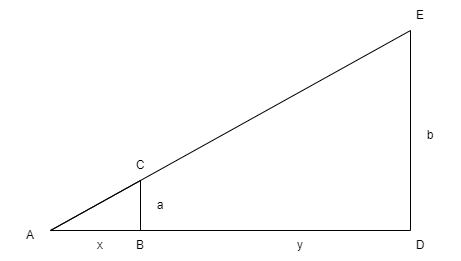
\includegraphics[scale=0.6]{similar_triangle.png}
        \end{figure}Given the above figure. $ACE$ and $ABD$ are straight lines and $BC//DE$. Also known that $AB=x$, $BD=y$, $BC=a$ and $DE=b$.\begin{enumerate}
            \item Prove that $\triangle ABC\sim\triangle ADE$.
            \item Find $a$ in terms of $b,x,y$.
            \item If $\angle CAB = 30^\circ$, with $b=10$ and $y=7\sqrt{3}$, find the area of $\triangle ABC$.
        \end{enumerate}
        \item Find the mean, mode, median of the following data: $$12,13,13,13,14,14,15,15,15,17,17,18$$
        \item Given a shooting board as following:\begin{figure}[H]
            \centering
            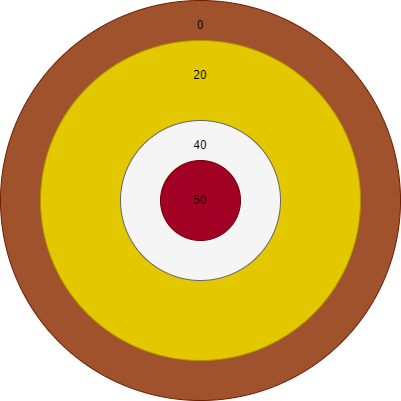
\includegraphics[scale=0.6]{shooting_board.png}
        \end{figure} It is given that the red zone is a circle of radius 5 cm, the white zone is a path of width 5 cm, the yellow zone is a path of width 10 cm, and the orange zone is a path of width 5 cm. Each zone owes the value written on the board. Suppose Owen is a shooter who has never missed any shots.\begin{enumerate}
            \item Find the probability for Owen to hit the red zone, the white zone, the yellow zone and the orange zone respectively. You may assume the chance of hitting every position on the board is equal.
            \item Find the expected value of each shot for Owen. 
        \end{enumerate}
    \end{enumerate}

\end{document}